\documentclass{article}
\usepackage[utf8]{inputenc}
\usepackage{graphicx}
\usepackage{blindtext}
\usepackage{subfiles}
\usepackage[colorlinks = false]{hyperref}
\usepackage[table]{xcolor}
\usepackage{rotating}
\usepackage{adjustbox}


\usepackage[TS1,T1]{fontenc}

\usepackage[
backend=biber,
style=authoryear,
citestyle=authoryear
]{biblatex}
\renewcommand*{\bibfont}{\footnotesize}
\usepackage[normalem]{ulem}
\usepackage{fancyhdr}
\pagestyle{fancy}
\fancyhf{}
\rhead{Measuring Rhetorical Similarity}
\lhead{Nicolai Berk}
\cfoot{\thepage}

\useunder{\uline}{\ul}{}

\addbibresource{refs.bib}

\title{Measuring Rhetorical Similarity with Supervised Machine Learning
\footnote{Replication materials are available via \href{https://github.com/nicolaiberk/SMLSE}{https://github.com/nicolaiberk/SMLSE}}
}
\author{Nicolai Berk}
\date{\today}


\begin{document}

\maketitle


\begin{abstract}
Recent advances in the application of supervised learning have shown how the method can be employed to measure polarization by assessing classifiers' accuracy. Building on these contributions, I propose a reconceptualisation to enable extended utilization of this approach. Focusing on predicted probabilites as a measure of rhetorical similarity, I validate supervised learning for the measurement of accommodation to radical right parties through established parties and politicians in Austria, Germany, and the Netherlands. Results indicate that the method produces valid estimates of parties' and speakers' rhetorical similarities to respective radical-right parties and outperforms existing similarity measures and scaling methods. I discuss possible further applications and limitations.\par \medskip

% add findings?

\textbf{Keywords:} measurement, rhetorical similarity, parliamentary debate, text analysis, supervised learning, machine learning, party competition, radical-right, political rhetoric.
\end{abstract}

\begin{center}
Word count: ca. 7,466
\end{center}

\section{Introduction}
\label{sec:Intro}
Political scientists are often interested in the rhetorical similarity of different sets of texts. For example, scholars of representation might be interested whether certain groups communicate distinctively in parliament (\cite{Pitkin1967}) or whether legislation is similar to demands voiced by interest groups (\cite{Gilens2014a}). Students of government formation and termination want to know which parties communicate most similar and are hence most likely to govern with each other (\cite{Gamson1961}), and when these coalitions are likely to break down (\cite{Lupia1995CoalitionTermination}). Public opinion scholars evaluate how the media or political groups left their mark on the current public discourse (\cite{Zaller1992}). Scientists interested in party competition might assess historical similarities between parties to judge whether one party filled a place abandoned by another (\cite{Kitschelt1986}), or whether one party moved towards another (\cite{Downs1957}). Knowing how similar MPs communicate allows to judge whether certain MPs are likely to leave their party (\cite{Hirschman1970}).\par

Despite the centrality of rhetorical similarities to political science research, existing approaches to measure it are limited. Scaling methods such as wordscore (\cite{Laver2003}) and wordfish (\cite{Slapin2008}) place labels\footnote{I define 'labels' as meta-information about documents (such as authorship), which allows to group said documents into corpora. A corpus (plural: corpora) is a group of documents.} in a one- (wordfish) or multi-dimensional space (wordscore), based on their word usage. These measures were designed for measuring ideological positions, not similarities, as they cannot precisely estimate the similarity of a given document \textit{with} a corpus. As such, they measure a latent dimension to be interpreted by the researcher, not a stable, pre-defined construct (\cite{Goet2019}). Simpler similarity measures, such as cosine similarity, are designed to assess literal identity of single documents, however perform badly for meaningful assessments (\cite{Prasetya2018}). To my knowledge, no specified method to estimate the rhetorical similarity of groups exists at the time of writing.\par

To address this methodological gap, I propose the use of supervised learning to measure the similarity of a given document with a specified corpus. This approach builds on an existing method to assess the similarity between groups using classifier accuracy (\cite{Peterson2018}), but moves the focus to predicted probabilities as a substantive similarity measure. This enables to provide a precise similarity estimate for each document, based on its word use. In the next section, I briefly discuss the relevance of rhetorical similarity and the capability of existing methods to capture it. Afterwards, I explain how supervised learning can be used to estimate rhetorical similarity step by step. Using parliamentary speeches from Austria, Germany, and the Netherlands, I then provide evidence indicating that the indicator is able to distinguish radical-right parties in line with theoretical expectations and produce valid estimates of similarity to the radical-right for established parties and speakers. The last section compares these estimates with wordfish and cosine similarity estimates and shows that the supervised method returns more meaningful, precise and efficient results.\par


\section{Estimating rhetorical similarity}

The logic of my approach builds on the idea that language is indicative of the way humans perceive and understand their surrounding world. In this view, rhetorical similarities, i.e. the shared dictionaries and figures of speech to describe reality, are symptoms of similarities in mental representations and cognitive processes (\cite{Lakoff1980Metaphors, Pennebaker2003}). This extends to the political realm: people who talk about political topics in similar ways, using the same words, should have similar perceptions of which issues are at stake and share common mental representations of these issues.\par

A measure of such rhetorical similarity should have several properties to be considered valid and useful. First, such an indicator should reflect a given document's similarity to other documents. The resulting estimate should then be informative about which corpus a document is likely to belong to. As corpora of interest to political scientists are often very large, the method should be scalable and fast to apply. Ideally, its application would not presuppose an understanding of the language through the researcher, but allow for 'language-blind' application in different contexts. However, \textit{if} the researcher is able to understand the language, meaningful information about what drives similarities and distinctiveness of documents is desirable. \par


\subsection{Existing similarity measures}

Several existing methods could be used to measure rhetorical similarity. A rather simple approach to similarity - cosine similarity - places documents in a multidimensional space. Every word constitutes a dimension ('feature') and the number of times that word was used defines the placement of a document on that dimension. Each document is then represented by a vector in high-dimensional (word) space. The cosine of the angle between those two vectors indicates how similar the word use in two given documents is, independent of the documents' length\footnote{That is, two documents containing words $a$ and $b$ are considered identical, as long as they contain them in equal shares.} (\cite{Similarity2007a}).  Similarly simple, Jaccard similarity compares the words used in two given documents and returns the share of common words (independent of how often they are used) relative to all words used in the documents (\cite{Jaccard1912}).\par

Methods like cosine and Jaccard similarity are designed for literal comparison of single documents. This kind of lexical similarity is interesting in several domains of social sciences, for example whether the release of specific documents affected political speech (\cite{Similarity2007a, Hager2020}). However, political scientists are usually interested in the similarity of groups, such as political parties, or identities such as gender. Additionally, each feature (word) has the same weight - the differing importance of words cannot be modelled. As a result, these measures are well designed to measure literal similarity, but do not perform well when similarity in meaning is concerned (\cite{Prasetya2018}).\par

Rhetorical similarity could also be assessed using scaling methods. Prevalent in political science for the measurement of the ideological placement of texts, these methods estimate underlying dimension(s) explaining differences in word use and scale the documents on this dimension. This happens either using labelled reference texts (wordscore; \cite{Laver2003}), or using certain assumptions about the distribution of words (wordfish; \cite{Slapin2008}). Both methods also allow researchers to assess the placement of individual terms, enabling to detect more meaningful differences between corpora inductively. \par

Wordscores are highly dependent on the reference documents selected and labelled by the researcher. This not only reduces the amount of processed information to the reference texts, but possibly introduces subjective bias. Additionally, the correct estimation and interpretation of Wordscores is not always straightforward (\cite{Lowe2008}). Less tedious is the application of an unsupervised method for scaling: Wordfish extracts the primary underlying dimension explaining word use by estimating it as a function of the length of a document, the frequency of a word in all documents, and estimated weights for words and groups, such as parties. The method then re-estimates this model - starting with arbitrary values - until the model fit is maximised (\cite{Slapin2008}). It also fits the model on the entire data, which substantially increases the variation taken into account.\par

Nevertheless, it also builds on the assumption that the differences in word use between the documents are indicative of the main (ideological) differences between labels (e.g. parties). However, the factors extracted are not necessarily indicative of those differences, which might sometimes result in failure to distinguish labels of interest (\cite[292f]{Grimmer2013TextASData}). Most importantly, both methods are designed to extract the primary dimension structuring differences in word use, not similarity to a corpus. This means that differences in scaling are indicative of placements on an often hard to interpret underlying dimension, not a clearly defined and easy-to-interpret construct.\par

All discussed approaches reflect similarities in word use, are highly scalable, and (with the exception of wordscores) allow an application without knowledge of the particular language texts are written in. However, these methods have major shortcomings for the assessment of the similarity of documents to corpora, either because they do not account for meaningful differences or are not designed to estimate such similarities. An indicator that mitigates these problems should focus on the differences between labels. Moreover, without relying on subjective judgement or hard-to-interpret factors, it should estimate precise similarity scores while maintaining simplicity of application, scalability, and language-blindness. Such an indicator is presented in the next section.\par

\subsection{Using supervised machine learning to measure rhetorical similarity}
\label{sec:method}

Instead of estimating similarities of single documents or underlying factors, differences in word use can also be exploited through machine learning to predict the likelihood that a document belongs to a certain corpus. Classic machine learning applications such as authorship studies use this approach to estimate the likelihood that an unlabelled document belongs to a given label (e.g. is authored by a specific person; \cite{Mosteller1963}). \citeauthor{Peterson2018} (\citeyear{Peterson2018}) invert this logic: instead of using labelled documents to extrapolate to unlabelled documents, they measure how similar two groups producing texts are, using only labelled data. That is, for each observed period (in their case, the legislative period), they obtain a classifier accuracy, which is informative of how well the groups of documents (e.g. speeches from two parties) can be distinguished, based on their word use. From that, they infer how similar the groups are to assess how polarised the British parliament was in a given legislature (for similar applications, see \cite{Gentzkow2019, Goet2019}).\par 

I extend this more descriptive application of supervised machine learning to generate an indicator of similarity to a given corpus for each document. Rather than assessing classifier accuracy and obtaining one data point per period, I focus on predicted probabilities as a substantive quantity of interest. These allow the precise estimation of the similarity of each single document to a given corpus (e.g. speeches by a specific party). The method is language-blind (as it only needs to know the frequencies of words) and highly scalable (ten thousand or one million speeches need the same amount of code and human labour). If researchers speak the language, they can assess the best predictor words to learn about the quality of the rhetorical differences. Most importantly, it measures an easy-to-interpret dimension, defined by the researcher. \par

Summarised, the method I propose works as follows: a classifier is trained on the full data\footnote{I diverge from the applications by \cite{Peterson2018} and \cite{Goet2019} in that I train the classifiers on the full data, reflecting the descriptiveness of the application (rather than inferring to unlabelled texts) and taking into account the entire available data. The section on comparative performance compares estimates from the full data to those trained on a subset of the data.} to estimate whether a text carries a certain label (e.g. is authored by a certain party). This results in a model where each word is assigned a correlation coefficient, indicating it's association with this label. Based on this model, the classifier assesses the likelihood that a text belongs to a label of interest. This predicted probability is estimated \textit{based on the similarity of word use} to the texts with this specific label. Thus, the likelihood that a text belongs to the category of interest is itself a similarity measure. Even though the researcher knows whether a document belongs to a certain label or not, the specific word use can still resemble that of a 'typical' document from that set more or less. The predicted probabilities of the bag-of-words model reflect this variation. \par

The list below outlines the application procedure. It should help readers understand and evaluate the estimates, but also guide researchers in their efforts to employ this indicator for their own purposes. \medskip

\begin{enumerate}
    \item \textbf{Select a Classifier} \newline Although the similarities are only interpretable relative to other estimates, it is desirable to use a classifier that is able to distinguish well between the labels in order to extract meaningful information. To that end, one should compare the performance of a number of pre-processing steps and classifiers before deciding which to use. Following \citeauthor{Peterson2018}, I do not remove stopwords from a pre-defined list, but very frequent as well as rare terms to avoid overfitting (\citeyear{Peterson2018}). This is more context-specific and should thus also be more neutral in its impact (see \cite{Schoonvelde2019a} for a discussion of this issue). Beyond that, the researcher should compare the performance of classifiers when using stemmed and unstemmed text, raw term counts and counts weighted by overall document frequency (tf-idf), as well as different classification algorithms (\cite{Denny2018}).\par 
    Training classifiers several times on subsets of the data and assessing average performance (cross-validation) minimises the risk of overfitting in the selection process (\cite{Breiman1989}). This is especially relevant as textual data suffers from finite-sample bias, meaning the speakers can only choose so many words from a huge dictionary of possible words. This bias might result in the over-estimation of partisan differences simply due to chance\footnote{Three steps are taken to reduce this problem: first, a bag-of-words approach is used (whereas \citeauthor{Gentzkow2019} used bi-grams), severely de-creasing the feature space. Second, the five-fold cross-validation ensures that a classifier which performs well on different subsets of data is selected, thus reducing the chance to overfit. Third, very rare terms (being used in less than five speeches within a period) are excluded, thus again reducing the likelihood that certain rare words discriminate between the parties just by chance.} (\cite{Gentzkow2019}).  \par
    Deviating from \citeauthor{Peterson2018}, I select a classifier once and apply it to the entire data. As these authors have shown, one can barely distinguish results from different classifiers (see Appendix D in \cite{Peterson2018}). My approach values the relative comparability of the estimates over the slight improve in predictive performance. The latter has little use for this descriptive application of supervised learning. \par
    \item \textbf{Balance the data} \newline Classifiers perform sub-optimal on imbalanced data. This could result in better performance for larger sets and worse performance for smaller sets of documents, rendering the latter documents more similar than they actually are. To avoid this, the data must be weighted. The final training set then consists to 50\% of speeches carrying the label of interest. This is additionally important if similarities of different subgroups should be compared. Then all subgroups should be weighted such that they represent equal shares and the label of interest contributes 50\% of all data.  \par
    \item (if necessary) \textbf{Divide the data into time-periods} \newline Sometimes, researchers might want to assess similarities across time. However, the use and meaning of words change across time. To address this issue, the data can be divided into subsets across time (e.g. a legislative session or presidential term). Training one classifier per time-period controls for changing language.\par
    \item \textbf{Fit the classifier(s) and estimate predicted probabilities} \newline The selected classifier is fitted to the over-sampled data (think of a regression where each word is an independent variable predicting the label, e.g. party membership of the speaker), returning coefficients\footnote{Note that some classifiers might not return coefficients nor use regression. This example was chosen for its perspicuity.} for each word based on the correlation with the label of interest (e.g. radical-right authorship). Using this classifier, predicted probabilities are estimated for each speech. The higher the likelihood estimated, the more similar the word use in the document to the word use in documents carrying the label of interest.\par 
\end{enumerate}



\section{Empirical data}
To demonstrate the application and validity of these similarity estimates, I employ the ParlSpeech dataset of parliamentary speeches (\cite{Rauh2020}) to study the rhetorical similarities of parties and speakers with the radical-right. The accommodation of radical-right parties by mainstream parties has inspired a vast literature and constitutes a major area of research on party competition (see e.g. \cite{Arzheimer2009, Bale2010e, Dahlstrom2012a, Harmel1997a, Krause2019accomodation, Meguid2005, Schumacher2014a, Spoon2020a, VanDerBrug2005b, VanSpanje2010, Wagner2017}). I selected the cases of the Austrian \textit{Nationalrat}, Germany's \textit{Bundestag}, and the \textit{Tweede Kamer} of the Netherlands. The Dutch and Austrian cases allow to make a historical assessment of the similarity of mainstream parties and speakers to the radical-right, as their party systems include radical-right parties for at least the past twenty years. Germany, on the other hand, has only recently witnessed the rise of the radical-right, but represents a much-studied case (see \cite{Arzheimer2019}: 2-5 for a review).\par

Using the \texttt{Scikit-Learn} package for python (\cite{Pedregosa2011}), I develop a classifier to estimate whether a text is authored by a radical-right party (Germany: AfD; Austria: FPÖ, BZÖ; Netherlands: LPF, PVV, FvD). I use the German data for classifier selection. After removing very infrequent and very frequent terms as well as punctuation from the texts, I train three different models (Logistic Regression, Multinomial Naïve Bayes, Support Vector Machine) on stemmed and un-stemmed text, quantified as either raw document counts, or weighted by the terms' inverse frequency across documents. This results in 3x2x2 = 12 different classifiers. I use five-fold cross-validation to choose a classifier that performs well. The logistic regression on inverse-document-frequency-weighted un-stemmed texts produces the most desirable results ('predicting' single speech authorship\footnote{Note that only just below 15\% of speeches were AfD speeches.}: accuracy 0.87, recall 0.59, precision 0.62) and is hence chosen as the classifier of interest for all applications (see appendix A for a comparison of the classifier performances). Bi- and tri-grams did not substantially affect these estimates nor improve interpretability of the best predictors and were hence excluded of the analysis. The training data was over-sampled using the SMOTE-algorithm from the \texttt{imblearn}-package (\cite{Lemaitre2017})\footnote{The synthetic minority oversampling technique (SMOTE) uses a 'nearest-neighbour'-approach to generate additional, synthetic cases. This method performs superior to other methods of balancing data (\cite{Chawla2002}).}. For the classification of Austrian and Dutch speeches, I train one classifier per legislative session, thus controlling for changing language across time. The German parliament saw the re-emergence of the radical-right only in 2017, therefore only one classifier is trained for this data (which ends in December 2018). \par


\section{Validity}
After preparing the similarity estimates as described, I assess their validity using three major tests. First, I assess the correspondence of the measure to the underlying construct of 'party-ness' (content validity) by assessing the best predictor words distinguishing the respective radical right party from all parties in that party system. Subsequently, I will use data from Austria and the Netherlands to show that radical-right and centre-right parties become more similar when governing together. After that, I will turn to individual estimates of speakers and assess whether the classifier places individuals that exited the radical right party in Germany differently. The last case examines the tranformation of Geert Wilders, a former member of the liberal party in the Netherlands, who would later form a major radical-right party. The estimates perform according to expectations in all cases and thus strongly corroborate the validity of the method.\par



\subsection{Content validity: best predictor words}

Radical-right parties are usually defined based on their distinctive policy positions. These parties are nationalist and hold especially conservative cultural as well as authoritarian positions. Additionally, they often communicate with populist rhetoric, including anti-elitism and people-centrism (\cite{Mudde2007}). Table \ref{tab:bpws} shows the words most positively (red) and negatively (turquoise) correlated with radical-right authorship. These words are the best predictors to distinguish the radical-right parties (FPÖ; AfD; PVV/FvD) in the most recent legislative period in the data (ending in Dec 2018 in DE \& AT, Jul 2019 in NL), out of all words in the model. \par

Considerable differences exist in the rhetoric distinguishing radical-right parties in these three countries. The AfD in Germany is foremost differentiated by its aversion to gender-inclusive language, which the party criticises as ‘gender-madness’\footnote{See \url{https://afdkompakt.de/tag/genderwahn/}}. It also displays heightened reference to itself, Germany (in line with its nationalist ideology), and the government (being the largest opposition party), compared to other parties. Its members address the parliament with ‘ladies and gentlemen’, not the male and female forms of ‘colleagues’. The use of causal adverbs ('therefore', 'hence')\footnote{This is particularly interesting, as such causal language seems to correlate with a number of psychological states, most importantly analytic thinking  (\cite{Pennebaker2003, Pennebaker2011}).} and reference to ‘democrats’ is also less found in AfD-authored speeches. \par

\begin{table}[ht!]
\centering
\begin{tabular}{|l|l|l|}
\hline
\textbf{Germany}                         & \textbf{Austria}            & \textbf{The Netherlands} \\ \hline
\rowcolor[HTML]{c41200} 
citizen/s {[}m{]}                        & honoured                    & immigration              \\ \hline
\rowcolor[HTML]{c41200} 
Merkel                                   & SPÖ                         & and so on                \\ \hline
\rowcolor[HTML]{c41200} 
german                                   & once                        & Islam                    \\ \hline
\rowcolor[HTML]{c41200} 
AfD                                      & patients  {[}m{]}           & PVV                      \\ \hline
\rowcolor[HTML]{c41200} 
Germany                                  & colleague {[}f{]}           & Islamic                  \\ \hline
\rowcolor[HTML]{c41200} 
old-parties                              & just {[}temporal{]}/precisely & Brussels                 \\ \hline
\rowcolor[HTML]{c41200} 
here                                     & Hohes {[}as in 'Hohes Haus'{]} & possible                 \\ \hline
\rowcolor[HTML]{c41200} 
government                               & years                       & immigration policy       \\ \hline
\rowcolor[HTML]{c41200} 
much                                     & population                  & illegal immigrants       \\ \hline
\rowcolor[HTML]{c41200} 
thanks                                   & Social Democracy            & hate-speech paragraph    \\ \hline
\rowcolor[HTML]{c41200} 
ladies                                   & appropriate                 & sign                     \\ \hline
\rowcolor[HTML]{c41200} 
thank you                                & Kern (SPÖ)                  & animal police            \\ \hline
\rowcolor[HTML]{c41200} 
gentlemen                                & Pilz                        & house-keeping            \\ \hline
\rowcolor[HTML]{c41200} 
employees                                & sector                      & gigantic                 \\ \hline
\rowcolor[HTML]{c41200} 
\cellcolor[HTML]{00BFC4}soldiers {[}f{]} & also                        & discount                 \\ \hline
\rowcolor[HTML]{c41200} 
\cellcolor[HTML]{00BFC4}state secretary  & federal minister {[}m{]}            & bene                     \\ \hline
\rowcolor[HTML]{c41200} 
\cellcolor[HTML]{00BFC4}warmly           & colleague {[}m{]}           & status holders           \\ \hline
\rowcolor[HTML]{c41200} 
\cellcolor[HTML]{00BFC4}important        & perhaps                     & heaven’s sake            \\ \hline
\rowcolor[HTML]{00BFC4} 
coalition agreement                      & \cellcolor[HTML]{c41200}committee & Kops {(}PVV{)}           \\ \hline
\rowcolor[HTML]{00BFC4} 
last                                     & colleagues {[}m{]}          & consideration            \\ \hline
\rowcolor[HTML]{00BFC4} 
therefore                                & Kurz                        & At the same time         \\ \hline
\rowcolor[HTML]{00BFC4} 
the left                                 & citizens {[}f{]}            & agreements               \\ \hline
\rowcolor[HTML]{00BFC4} 
colleagues                               & dear                        & diligent                 \\ \hline
\rowcolor[HTML]{00BFC4} 
hence                                    & motion                      & advised against          \\ \hline
\rowcolor[HTML]{00BFC4} 
need                                     & humans                      & mister                   \\ \hline
\rowcolor[HTML]{00BFC4} 
citizens {[}f{]}                         & minister {[}f{]}            & look                     \\ \hline
\rowcolor[HTML]{00BFC4} 
democrats                                & FPÖ                         & Agema {(}PVV{)}          \\ \hline
\rowcolor[HTML]{00BFC4} 
say                                      & federal minister {[}f{]}                      & bright                   \\ \hline
\rowcolor[HTML]{00BFC4} 
think                                    & colleagues {[}f{]}          & predominant              \\ \hline
\rowcolor[HTML]{00BFC4} 
colleagues {[}f{]}                       & ÖVP                         & Baudet {(}FvD{)}         \\ \hline
\end{tabular}
\caption{Thirty best predictor words increasing (red/dark/top) and decreasing (turquoise/light/bottom) likelihood of radical-right authorship for Germany, Austria, and the Netherlands. Squared brackets indicate gender, round brackets note the party affiliation of specific names.}
\label{tab:bpws}
\end{table}

As the Austrian FPÖ was in government at the time, it makes sense that it is distinguished from other parties by reference to the opposition (the social democrats of the SPÖ are the main opposition party) rather than the government, including the reference to Vienna, a stronghold of the social democrats much criticised by the radical- and centre-right. It also prefers to address the parliament as ‘ladies’ and ‘gentlemen’ rather than ‘colleagues’. One of the major projects of the FPÖ-led health ministry was a reform of the health sector, which explains the reference to 'patients'. Referring to members of the government in female form decreases the likelihood of radical-right authorship (similar to the German AfD), as does reference to ‘humans’ and addressing the house ‘warmly’.\par

Lastly, and differing from their German and Austrian equivalents, the Dutch FvD and PVV are distinguished primarily by reference to immigration and Islam. These parties' rhetoric refers to 'immigration', 'Islam'/'islamic' and 'illegal immigrants' more than other parties, in line with their distinctively anti-immigration positions. Reference to 'Brussels' underlines the Eurosceptic position of these parties (\cite{ThePopulist2019}). Words like 'house-keeping', and 'discount' could refer to the Budget, where at least the FvD proposes tax cuts\footnote{See \url{https://www.fvd.nl/economie}}. Additionally, FvD and PVV make use of more informal ('and so on', 'heaven’s sake') and less nuancing language ('consideration', 'diligent', 'advised against', 'predominant'). As nouns are usually not gendered in Dutch, it is not surprising that gendered language is no predictor here.\par

The best predictor words are mainly in line with expectations about the political difference of radical-right parties in Germany, Austria, and the Netherlands. While the Dutch radical-right parties are primarily distinguished by their reference to immigration, as well as informal language, the German and Austrian radical-right parties resemble each other in their rejection of gendered language\footnote{However note that this does not mean that words about migration do not contribute positively to the German and Austrian estimates (in fact, they do). Instead, the 30 best predictor words offer a concise but ultimately superficial glimpse into the major differences between documents with the label of interest (radical-right authorhship) and all other documents.}. The at-the-time governing Austrian FPÖ displays increased reference to the opposition, while the German AfD is more likely to address the government. These findings also caution against a one-size-fits-all approach to pre-processing, as the rejection of gendered nouns would have remained hidden had I stemmed the words.\par


\subsection{Construct validity I: governing with the radical-right}
Coalition governments demand from the participating parties to make concessions in order to agree on shared policy goals. In parliament, these proposals need to be defended by the governing parties against criticism from the opposition. As a result, these parties should become more similar in their communication. The formation of coalition governments hence present a perfect case to validate the similarity estimates described above. \par

The Austrian case has seen the formation of three coalition governments between the conservative ÖVP and the radical-right FPÖ in 2000, 2003, and 2017. In 2000, the ÖVP managed to secure the chancellorship as the third-largest party by forming a coalition with the radical-right FPÖ. This broke the \textit{cordon sanitaire} formed by the social-democrat SPÖ and ÖVP to isolate the FPÖ after the takeover of right-wing populist Jörg Haider in 1986. The formation was met by strong internal and external criticism due to the FPÖ's radical xenophobic policy positions, resulting in diplomatic sanctions against the country and large-scale demonstrations. The coalition broke down in 2002 due to internal rifts within the FPÖ, forcing early elections. This time, the ÖVP emerged as the largest party and entered coalition talks with the Greens, which eventually broke down. A coalition government was again formed with the FPÖ. In April 2005, the FPÖ split, and the coalition continued with the split-off BZÖ until 2006 (\cite{Luther2010}).\par

The recent formation of the ÖVP-FPÖ coalition in 2017 was again met with domestic protests. After the experience of the so-called 'migration crisis' in 2015, immigration was the dominant topic in campaigns. ÖVP \textit{Spitzenkandidat} Kurz attacked the FPÖ's issue ownership, also taking  a restrictive position, especially surrounding the closure of the 'Balkan-route' for asylum seekers. This conveniently aligned these two parties' policies on this salient issue (\cite{Bodlos2018}). The data under study ends before the collapse of the government after the publication of the 'Ibiza-video' in 2019, showing FPÖ leaders Strache and Gudenus promising public contracts to a supposed Russian oligarch.\par 

Summarised, I expect the FPÖ to show higher resemblance with the ÖVP and the ÖVP to sound more alike the FPÖ while they govern together. This is especially true for the government formations in 2000 and 2017, where the ÖVP opted out of the mainstream coalition with the social democrats. \par

\begin{figure}
\begin{minipage}{\textwidth}
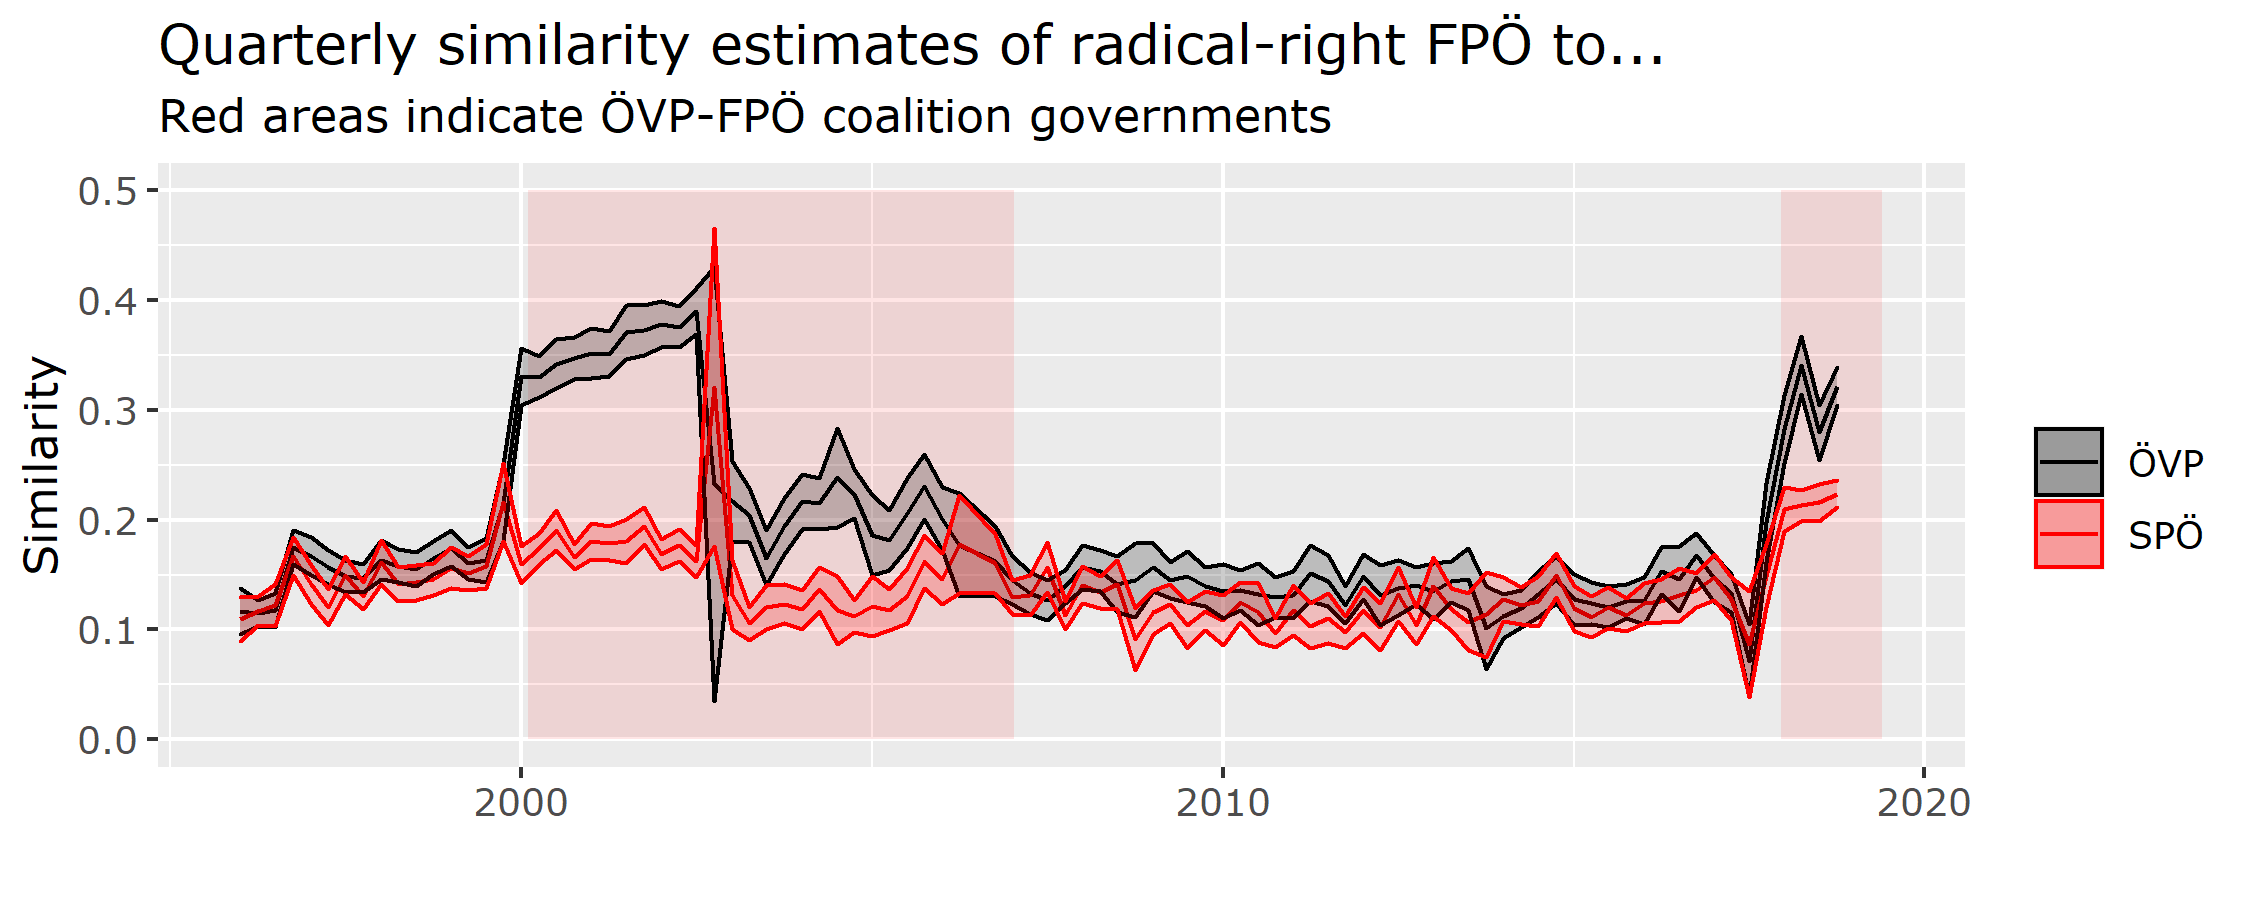
\includegraphics[width=\linewidth]{AT/vis/AT_fp_paper.png}
\end{minipage}
\hfill
\begin{minipage}{\textwidth}
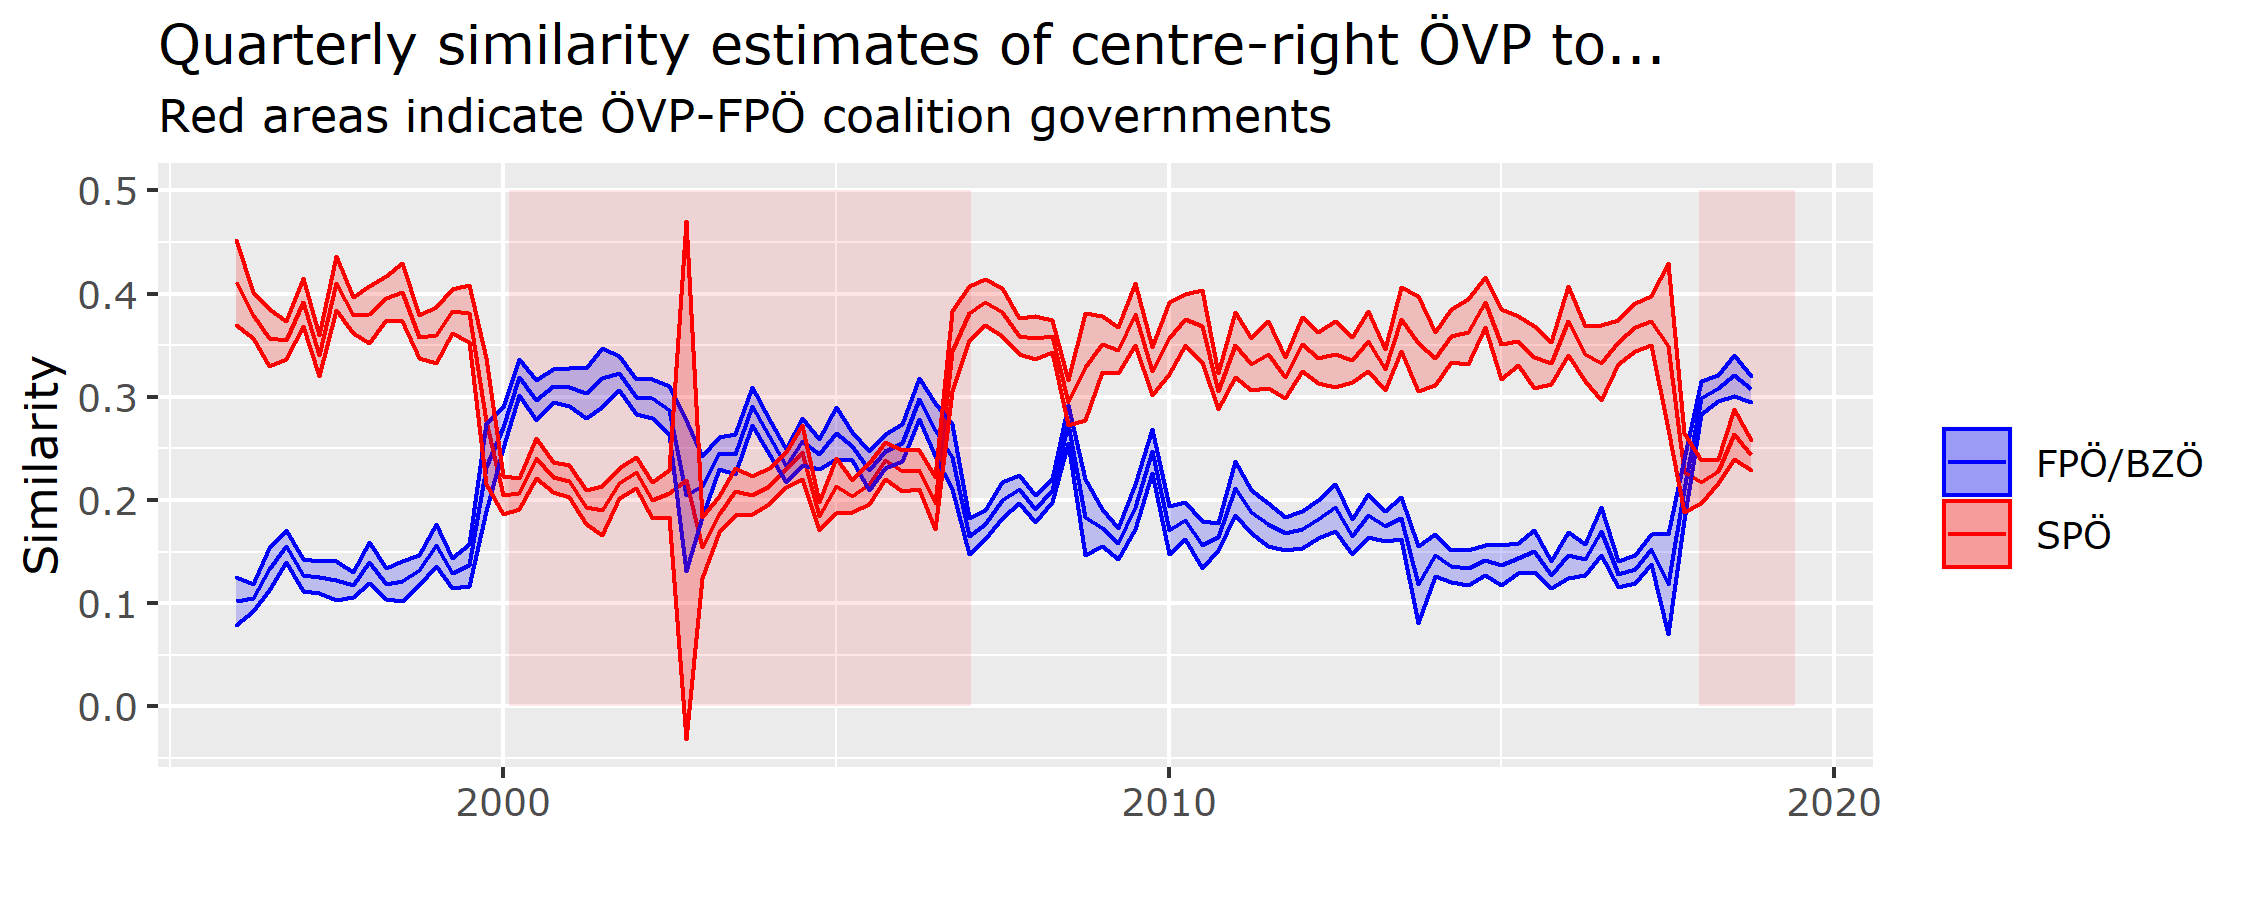
\includegraphics[width=\linewidth]{AT/vis/AT_vp_paper.png}
\end{minipage}
\caption{Quarterly average similarity to main competitors for centre-right and radical-right parties in Austria with 95\% confidence intervals.}
\label{fig:govs}
\end{figure}

Figure \ref{fig:govs} shows the quarterly mean estimates of the radical-right FPÖ (top) and centre-right ÖVP (bottom) towards each other\footnote{To improve interpretability, split-off BZÖ is considered part of the FPÖ here.}. To compare these estimates, the similarity to the third large party during this time, the social-democrat SPD, has been added to each graph. The red-shaded ares indicate the time in which FPÖ/BZÖ and ÖVP were governing together. The similarity estimates of the FPÖ indicate that after the first formation in 2000, the party's similarity to the centre-right ÖVP increased substantially from about 15\% to 30-40\%. After the breakdown of the first coalition following the internal rift in the FPÖ, the similarity decreases - the re-elected party seems to hold a distance. In 2017, a strong increase from ~10\% to ~30\% is visible again. Note that here, the similarity to the social democrat SPÖ also increased, which might indicate a moderation of the party.\par


In the estimates for the centre-right ÖVP (bottom graph figure \ref{fig:govs}), a similar pattern can be observed - most variance can be observed around coalition formations. In 2000, a similar strong move towards the FPÖ can be observed (10\% $\rightarrow$ 30\%), while the similarity with the SPÖ (with which the governed preceding the coalition with the FPÖ) strongly decreases from around 40\% to around 20\%. After the end of the coalition in 2006, the estimates 'flip' again, when the ÖVP enters a coalition with the social democrats. Lastly, the pattern from 2000 is repeated when the ÖVP again switches from a coalition with the social democrats to a coalition with the radical-right.\par

T-tests confirm a significantly increase in similarity of around 11.6 (FPÖ) and 11 (ÖVP) percentage points towards the respective other party when the two parties govern together, compared to all other time-periods in the data ($p<0.001$). Given an average similarity of 16\% when not governing together, this is a \textit{very} substantive difference. Similar findings can be reported for the Netherlands, see Appendix B.\par

More interesting patterns are visible. The FPÖ seems to moderate (spike in similarity to ÖVP \& SPÖ) before the first formation in 2000 - possibly related to Haider's efforts to calm worries about the parties' Nazi past (\cite{Luther2010}: 84); but more distinctive before the formation in 2018, where the ÖVP challenged the FPÖ's issue ownership on immigration, while the FPÖ underlined its 'orginalness' (\cite{Bodlos2018}). It is also visible how the FPÖ distinguished itself from the ÖVP after the 'Knittelfeld crisis' in September 2002, where party members challenged their leadership in open opposition to their course (\cite{Luther2002}). When the coalition broke down, the estimates briefly show a high similarity of the radical-right to the social democrats. The centre-right's estimates already seem to shift preceding the formations in 2000 and 2018, possibly signalling interest in coalition formation with the party. After the breakdown of the first ÖVP-FPÖ coalition in 2003, the similarity to the FPÖ hits a low, while the estimates of similarity to the SPÖ show a lot of uncertainty - this might have to do with considerations within the ÖVP to return to governing with the SPÖ, which openly supported this option (\cite{Luther2010}: 91). \par


These findings are in line with my expectations: parties communicate more similar to each other when in coalition. Interesting variation can be observed: parties accomodated to future coalition partners \textit{before} coalition formations, however intra-party factors seem to affect how close parties accomodate as well (see lower FPÖ estimates following Knittelfeld crisis, while still governing with ÖVP). These observations indicate possible starting points for future research with this method and underline the richness of the data.\par



\subsection{Construct validity II: leaving the AfD}

Beyond parties, the similarity or distinctiveness of particular speakers can also be of interest. I use two cases from Germany and the Netherlands to further validate the method's precision. In both cases, I have strong expectations about the placement of individual speakers. In Germany, six members of the AfD have since left the party, mainly due to the increasing strength of the far-right faction within the radical-right party (\cite{Steffen2020AfD}). Two of these members - one of whom was former party leader Frauke Petry - left within the first ten days following the election (\cite{LSE2018AfD}). As they were members of the party themselves, these members should obtain higher similarity scores than members of other parties\footnote{Note that the data contains no speeches by these two independent members preceding their exit, excluding a longitudinal analysis comparing their similarity before and after exit.}. Similarly, four members of the AfD who would leave the party later (outside of the observed time-frame) should obtain lower 'party-ness' scores, compared to loyal members of the AfD. \par

\begin{figure}
    \centering
    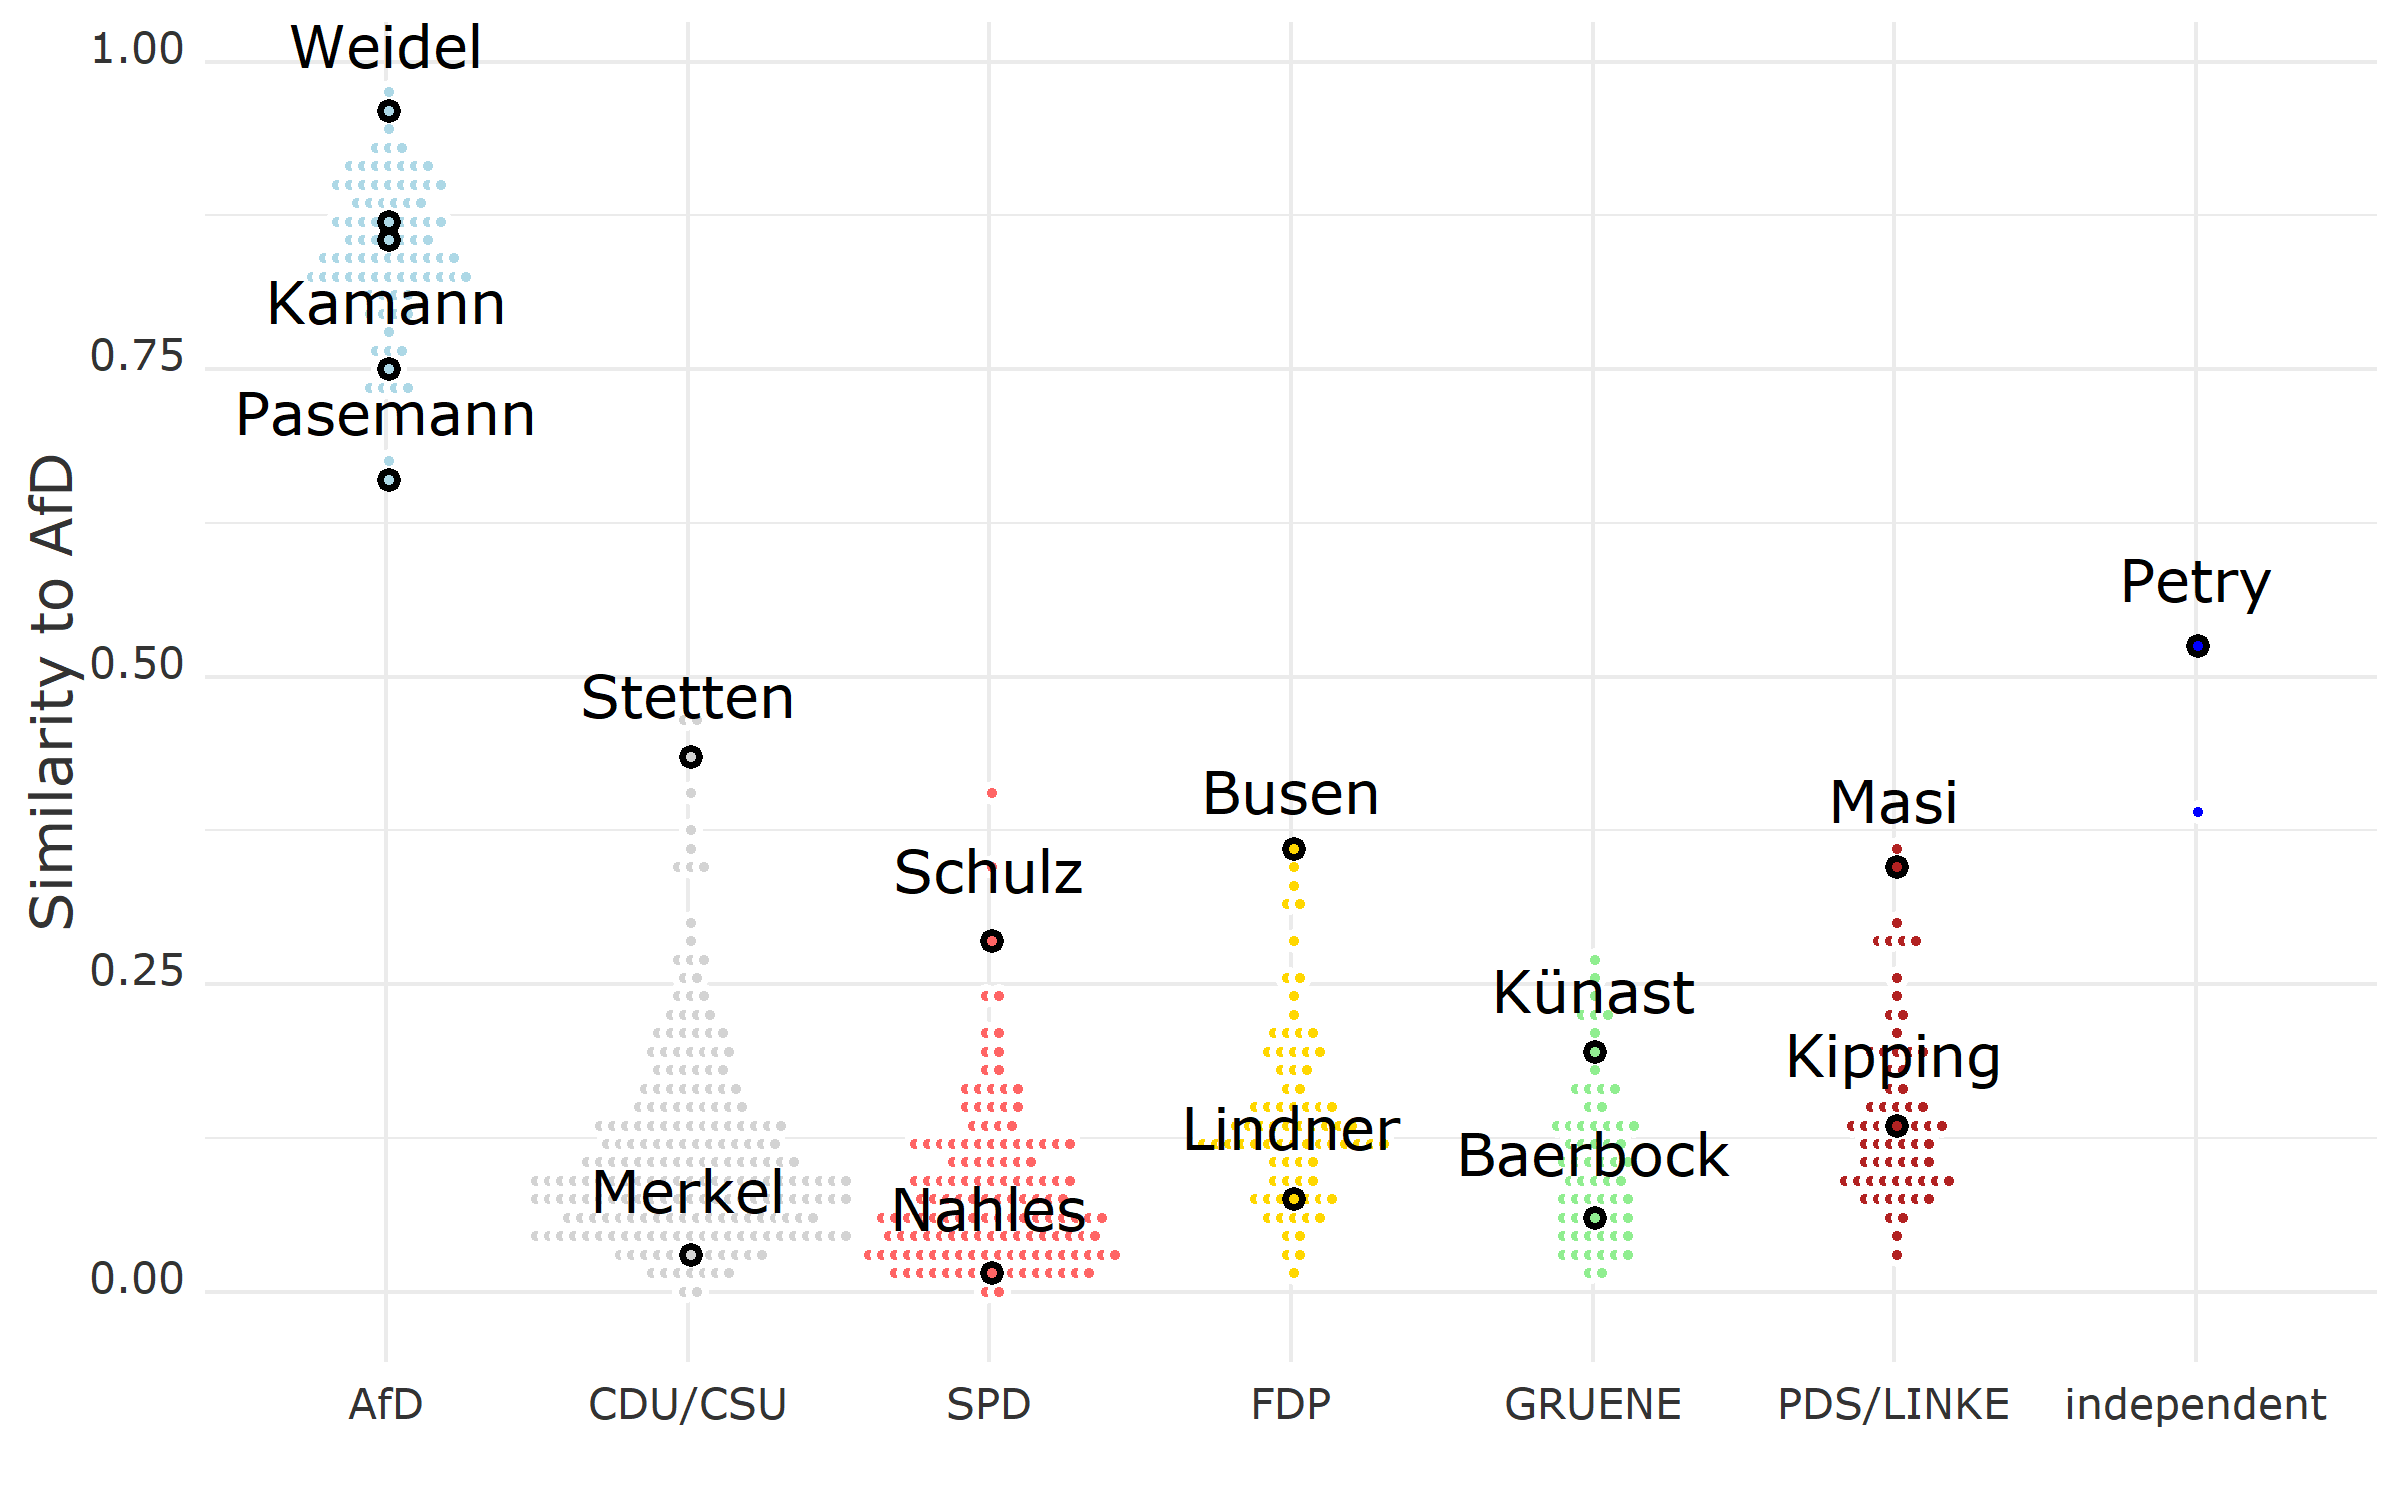
\includegraphics[width=\textwidth]{DE/vis/DE_speakers_PA.png}
    \caption{Estimated similarity to radical-right AfD for speakers of the current German Bundestag.}
    \label{fig:speakers}
\end{figure}

Figure \ref{fig:speakers} shows the mean estimate for each speaker in the current Bundestag. Each speaker is represented by a dot. The dot's position on the vertical axis indicates the speaker's similarity to the AfD, while its color and horizontal position indicate the speaker's party affiliation. The classifier discriminates speakers perfectly by assigning a probability greater than 0.5 for all AfD-members and a probability smaller than 0.5 to all speakers from established parties. In line with my expectation, the now independent former members of the AfD obtain rather high values (Frauke Petry: 52.6\%, Mario Mieruch: 39.3\%) and are located in between the AfD and the other parties. The mean estimate for all speeches by these two speakers is distinctive from all other parties. Despite being labelled not to be part of the AfD in the training data, the classifier correctly locates them in proximity of the AfD. \par

Uwe Kamann would leave the AfD five days after the observed period ends, on December 17th, 2018. His estimate is relatively low compared to his party, however several members obtain lower estimates. Lars Herrmann and Verena Hartmann, two other members that left the AfD, followed in winter 2019/2020, about one year after the data ends. In the data observed, the classifier still places them well inside their party (see two highlighted, unlabelled dots within the AfD). For these ex-members of the AfD, the expectations are not confirmed. It might be the case that they still move to the fringes of their party in the following year. The estimates for Frank Pasemann, the sixth member in the data to leave the party (and the only one to do so involuntarily), exemplify well how these similarity estimates can be interpreted. Pasemann was expelled from the AfD in August 2020, most likely as a result of anti-semitic statements and his proximity to members of neonazi- and radical-right associations\footnote{\cite{MDR2018Pasemann, MDR2020Pasemann}}. As the concept being measured is 'AfD-ness' (specified as the outcome category in the training data), the classifier assesses how well a speech fits into the corpus of AfD-speeches. As a result, Pasemann, who openly epresses views perceived as radical even by some fellow AfD-members, obtains lower estimates than other members of his party. Although far more detailed, the speaker estimates are in line with expectations, underlining the precision and validity of the method. \par

Beyond these specific members, all parties show considerable variation. The overall distribution of the two governing mainstream parties is skewed towards the lower end of the scale, with only few members in the tails with higher probabilities. This tail is more pronounced for the CDU/CSU. Among the conservatives, the measure seems to have an ideological component: those with a high probability of being members of the AfD also seem to have more conservative positions. While Angela Merkel is assigned a low similarity score (2.9\%), Christian von Stetten (43.2\%) and other more conservative members of the party are placed more closely to the AfD. Stetten is a vocal advocate of a conservative turn of his party under the leadership of Friedrich Merz (\cite{Weinzierler2019}), and has been affiliated with the conservative WerteUnion, which works towards a right-wing turn in German politics\footnote{He is quoted as a supporter (including a picture of his face) on the movements website: \url{https://werteunion.net/}}. Within the SPD, it is interesting that delegates from former industry regions in North Rhine-Westphalia and Eastern Germany like Dirk Vöpel (40.8\%), Detlef Mueller (34.9\%), and Martin Schulz (28.9\%) are assigned higher values compared to their party. However note that e.g. Martin Schultz is a fierce advocate against the radical-right\footnote{\cite{Tagesspiegel2018Schulz}}.\par

The estimates for the other opposition parties are somewhat more spread out than the two governing parties, but with similar tails towards the top. Within the FDP, Karlheinz Busen gets assigned the highest estimate of his party (35.3\%). His political positions revolve around agricultural matters \footnote{\url{https://karlheinz-busen.de/}}, which is an issue that the AfD is increasingly trying to mobilise on (\cite{Sueddeutsche2020AfD}).  Among the Linke, several members obtain rather high estimates, most prominently Fabio de Masi (34.6\%), a politician with a strong focus on EU-policy, where the party holds a Eurosceptic position\footnote{\url{https://www.fabio-de-masi.de/de/topic/15.eurokrise.html}} (as does the AfD; \cite{ThePopulist2019}).\par


\subsection{Construct validity III: The case of Geert Wilders}

In the Netherlands, the rise of the radical-right LPF in the early 2000s and the subsequent politicisation of immigration forced other parties to react to the issue (\cite{DeVries2012c, Pennings2003}). This proved a wedge issue for the liberal VVD, pitting the social-liberal faction around state secretaries Mark Rutte and Melanie Schultz against party members demanding a shift to the right, most famously Geert Wilders (\cite{VandeWardt2014, Vossen2011}). After being described as a likely candidate for party leadership of the VVD in the early 2000s (\cite[182]{Vossen2011}), Wilders developed an increasingly extreme anti-islamism from 2003 onwards (\cite[26]{Vossen2010}). This alienated him from the social-liberal wing of the VVD and the party's leadership, especially parliamentary group leader van Aartsen. In 2004, Wilders published a position paper together with his fellow VVD MP Gert-Jan Oplaat, calling for a right-wing turn in the VVD. It was speculated whether Wilders would join the LPF, which held similar anti-muslim and anti-immigration positions (\cite{Parool2004Wilders, Handelsblad2008Wilders}). After several calls by the leadership to follow the party line, he left the VVD to form the radical-right PVV, while the VVD took a more centrist course (\cite{Vossen2010, Vossen2011}). \par

As Wilders develops more anti-muslim positions, I expect him to become more similar to the LPF in the time preceding his exit, compared to other members of the VVD. This should especially be the case when compared to proponents of the social-liberal course of the VVD. Immigration-critical members of the VVD like Gert-Jan Oplaat (who co-authored the position paper with Wilders), Ayaan Hirsi Ali (who co-authored an op-ed with Wilders calling for a 'liberal Jihad'; \cite[183]{Vossen2011}) and Rita Verdonk (who later formed her own populist party \textit{Trots}) should be placed in proximity to the LPF, compared to the social-liberal wing. \par


\begin{figure}
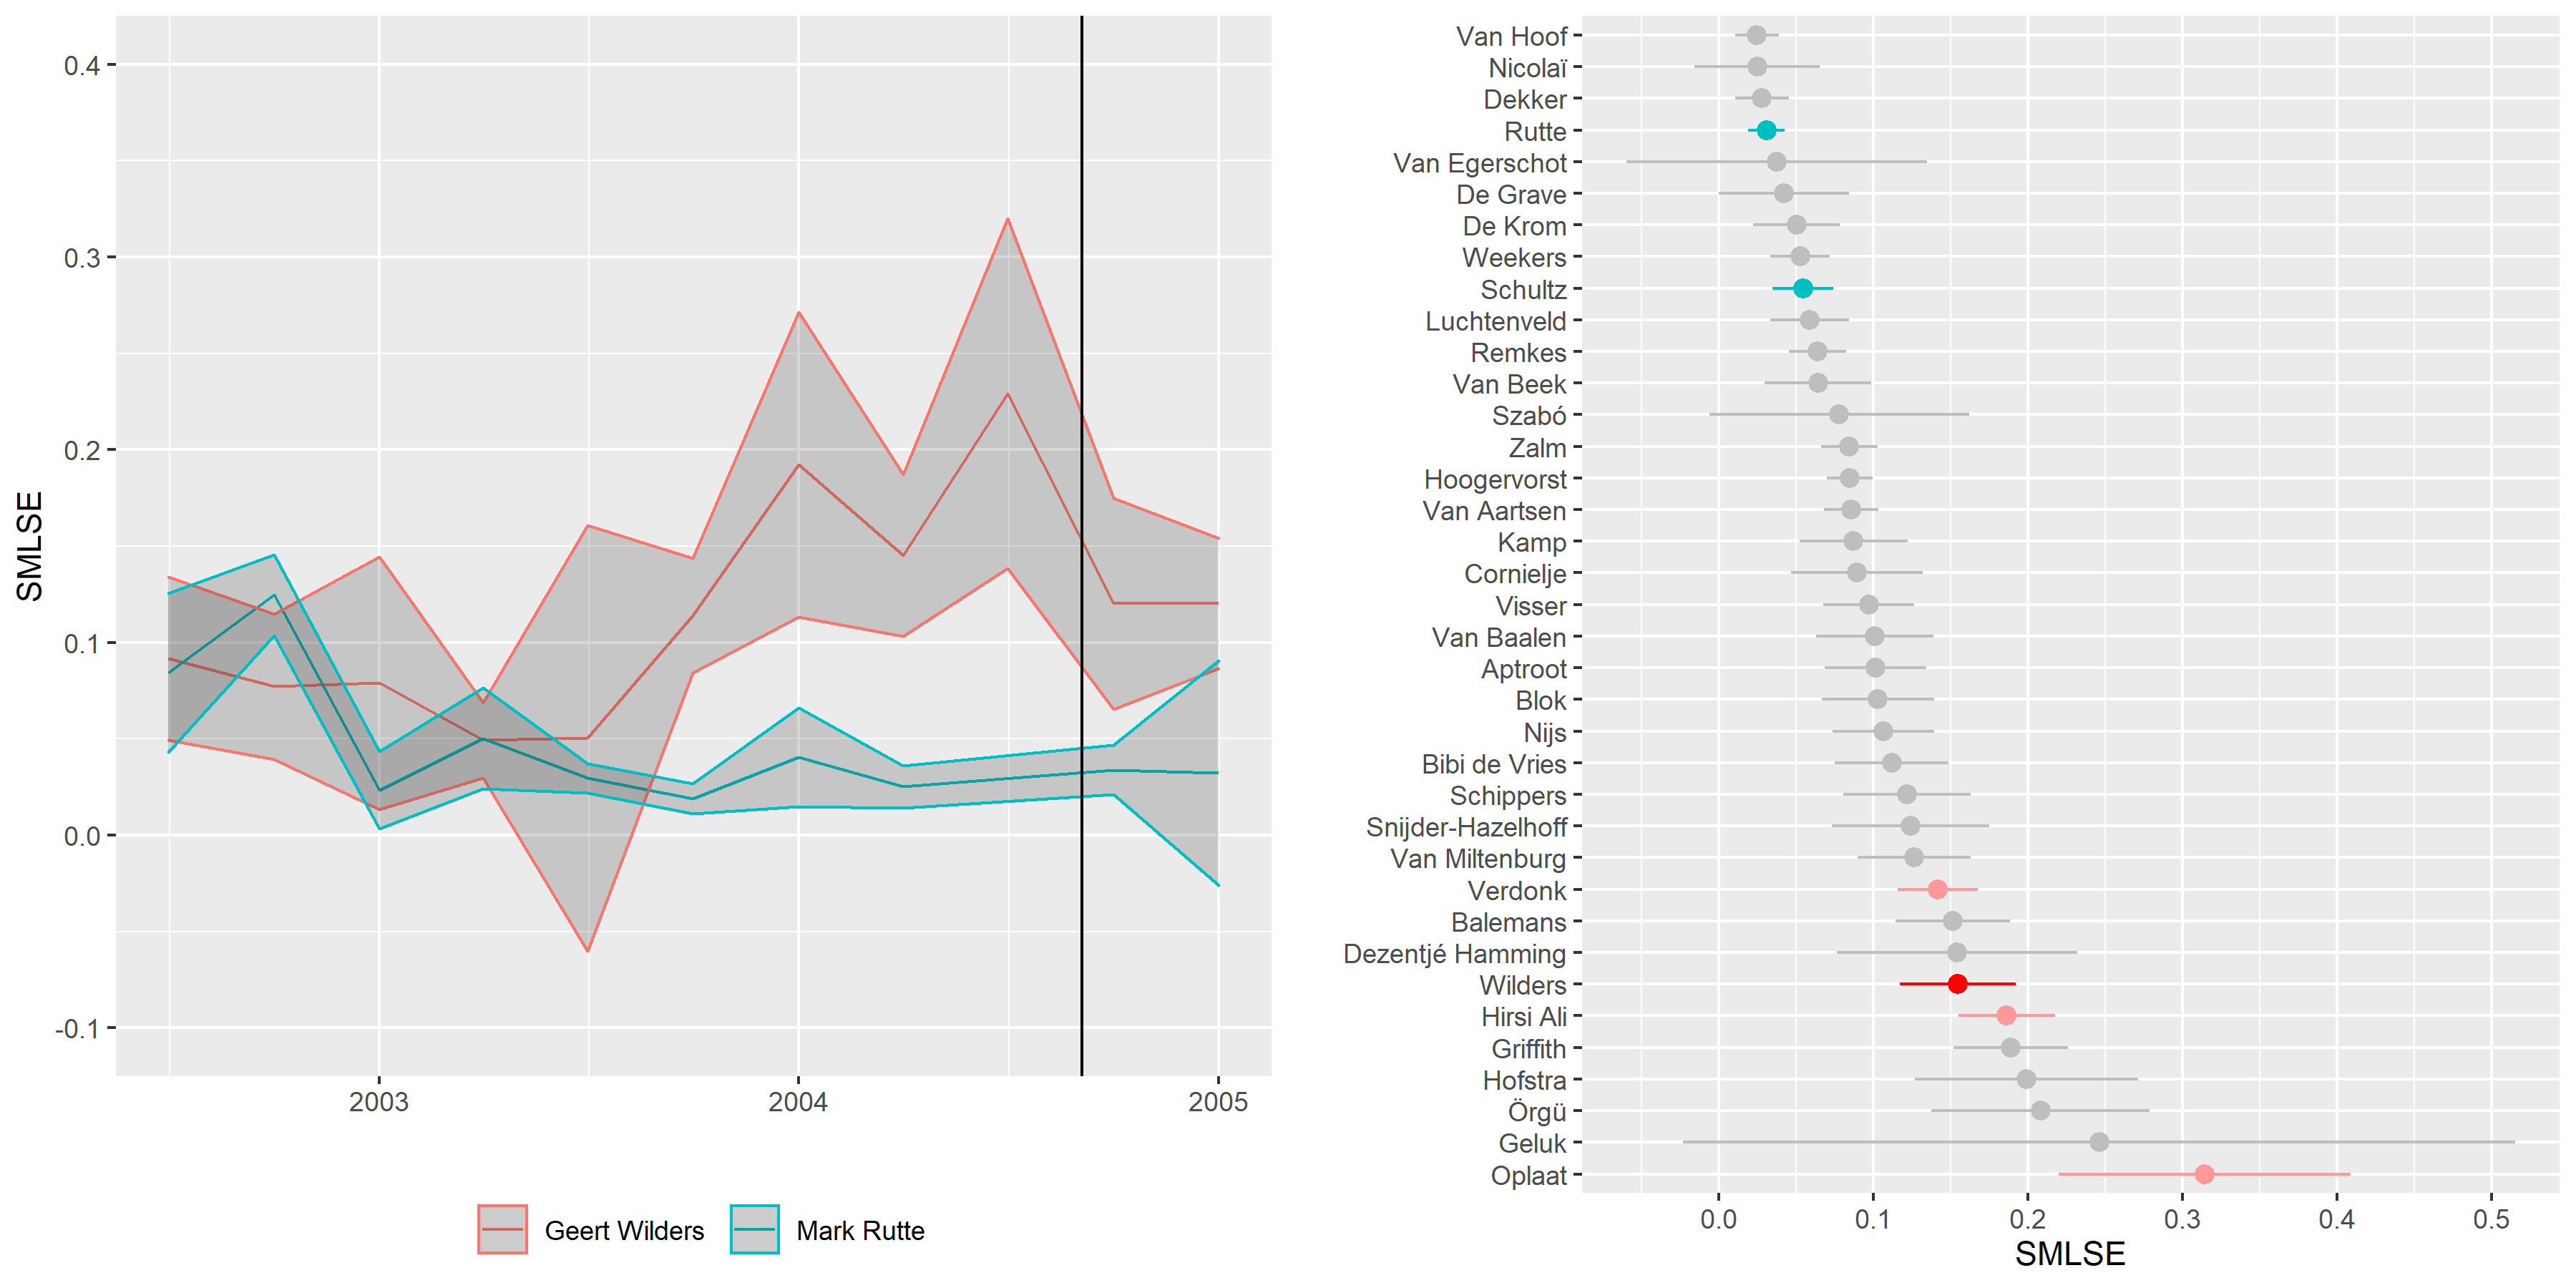
\includegraphics[width=\linewidth]{NL/vis/Wilders_both.png}
\caption{\textbf{Left}: monthly average similarity to the radical-right LPF for Geert Wilders and Mark Rutte in 2004. The vertical line indicates the date Wilders' left the party. \textbf{Right}: Placement of Wilders (red), compared to social-liberal (turquoise) and right-wing members (light-red) within the VVD in 2004, preceding Wilders' exit. Both graphs show the estimates with 95\% confidence intervals.}
\label{fig:wilders}
\end{figure}

The left graph in figure \ref{fig:wilders} shows the monthly mean similarity to the radical-right LPF for Geert Wilders and (at the time) more socially-liberal oriented Mark Rutte, from the first entry of the LPF until Wilders' exit. It is visible that in 2002 and early 2003, both estimates overlap at low levels. The classifier gives both speakers a 0-10\% chance to belong to the LPF. In line with my expectation, Wilders' estimate moves upwards from mid-2003, indicating higher similarity to the radical-right LPF. He briefly returns to lower levels of similarity, before a steep increase until September 2004 (the month of his exit), when the classifier assigns a likelihood of over 70\% that Wilders belongs to the LPF. This is especially extreme compared to the significantly distinctive estimate for Rutte at around 5\%. It seems that after the election, an issue sorting takes place, as Wilders embraces the LPF's position, while Rutte further distances himself (\cite{Carmines1986}). After his exit, Wilders' language changes again, becoming less alike the LPF, reflecting the fact that he would not join the LPF.  Summarised, Geert Wilders' divergence from the VVD from 2003 onwards is visible and significant in the supervised estimates.\par

Based on the scores alone, it is unclear what drives the increased similarity of Wilders' language to the LPF. The expectation is that the distinction should revolve around Islam and immigration, the major issue that Wilders' party mobilized on later (\cite{VanHolsteyn2011}). Disagreement on these issues was also reflected in the support agreement between VVD, CDA and PVV in 2010 (\cite[350]{Otjes2014}). I calculate each word's influence on Wilder's similarity score by multiplying the model coefficient with the (tfidf-weighted) word count from all his speeches between the second CDA-VVD-LPF government formation until his exit from the VVD in 2004. The 30 words with the strongest positive influence\footnote{See appendix D.} contain several terms related to Islam ('imam', 'mosques'), security ('AIVD'\footnote{AIVD is the Dutch intelligence service.}, 'Defense'), terrorism ('terrorists'), and muslim countries ('Algeria', 'Saudi', 'Arabia'), as well as 'Europe'. It seems that Wilders' increased similarity in this period is indeed related to his increased attention to Islam and terrorism.\par

The right side of figure \ref{fig:wilders} shows Wilders' placement compared to other VVD members in the period from January 2004 preceding his exit. In general, Wilders is placed relatively similar to the LPF, obtaining the 7th-highest estimate (20\%) of the 37 members covered by the data. Likewise, other members opposed to Islam and immigration (Hirsi Ali, Oplaat, Verdonk) obtain similarly high estimates (15.7\% -33.3\%), while the proponents of a social-liberal course (Rutte, Schultz) are assigned significantly lower estimates (3.2\%, 6.1\%). Assessing the VVD in 2004, the estimates correctly place social-liberal and more right-wing members within the party.\par 



\section{Comparative Performance}
The supervised similarity estimates conform to expectations in all described cases. Nevertheless, existing methods could be used to estimate rhetorical similarities. This section compares the supervised estimates of 'AfD-ness' for the current German legislature to cosine similarity and wordfish estimates. Cosine similarity is a relatively simple measure, which has seen political science applications (\cite{Similarity2007a, Hager2020}). It takes the cosine of the angle of two document vectors to assess their similarity. It equals one when the two compared documents are identical in their relative word usage and zero when the documents share no common words. Scaling methods like wordscore (\cite{Laver2003}) and wordfish (\cite{Slapin2008}) are more complex, but have become popular to estimate differences in party communication, mainly to place texts on an ideological scale. \par

\subsection{Cosine similarity}

Cosine similarity is calculated for each document, comparing it to all AfD-authored speeches, then taking the mean similarity score. This results in very low overall similarity scores, ranging between 0.04 and 0.05. Figure \ref{fig:comp} shows the mean values for supervised similarity estimates, cosine similarity, and wordfish for each party in the current German legislative period. While the AfD is clearly distinguished by the supervised estimates, there are only slight party differences for the cosine measure, with comparatively large confidence intervals. Cosine similarity is unable to distinguish AfD speeches, with the AfD only ranked \textit{third} in similarity to AfD speeches. This is in line with weak performance of this measure when meaning is relevant (as opposed to e.g. the detection of plagiarism, where literal similarity is relevant; \cite{Prasetya2018}).\par

The weak performance becomes more obvious once the measure is correlated with speech length: over 75\% of the variance in cosine similarity are explained by the length of the speech (Pearson's r = 0.87). It seems that the increased likelihood of a word to be included is the main driver of increased similarity here. The correlation of cosine similarity with the supervised measure is in fact weakly \textit{negative} (-0.17)\footnote{When using the log of the supervised estimates to normalise the distribution, this decreases to -0.36.}. AfD authorship is statistically unrelated to cosine similarity (correlation of -0.02). Calculating cosine similarity of these groups differently by first generating the average word count of AfD speeches and then calculating cosine similarity results in virtually identical results. I also calculated Jaccard\footnote{Jaccard similarity assesses the share of common words among all words used (it is unrelated to how often the words are used).} similarity with similarly weak performance.\par

\begin{figure}
    \centering
    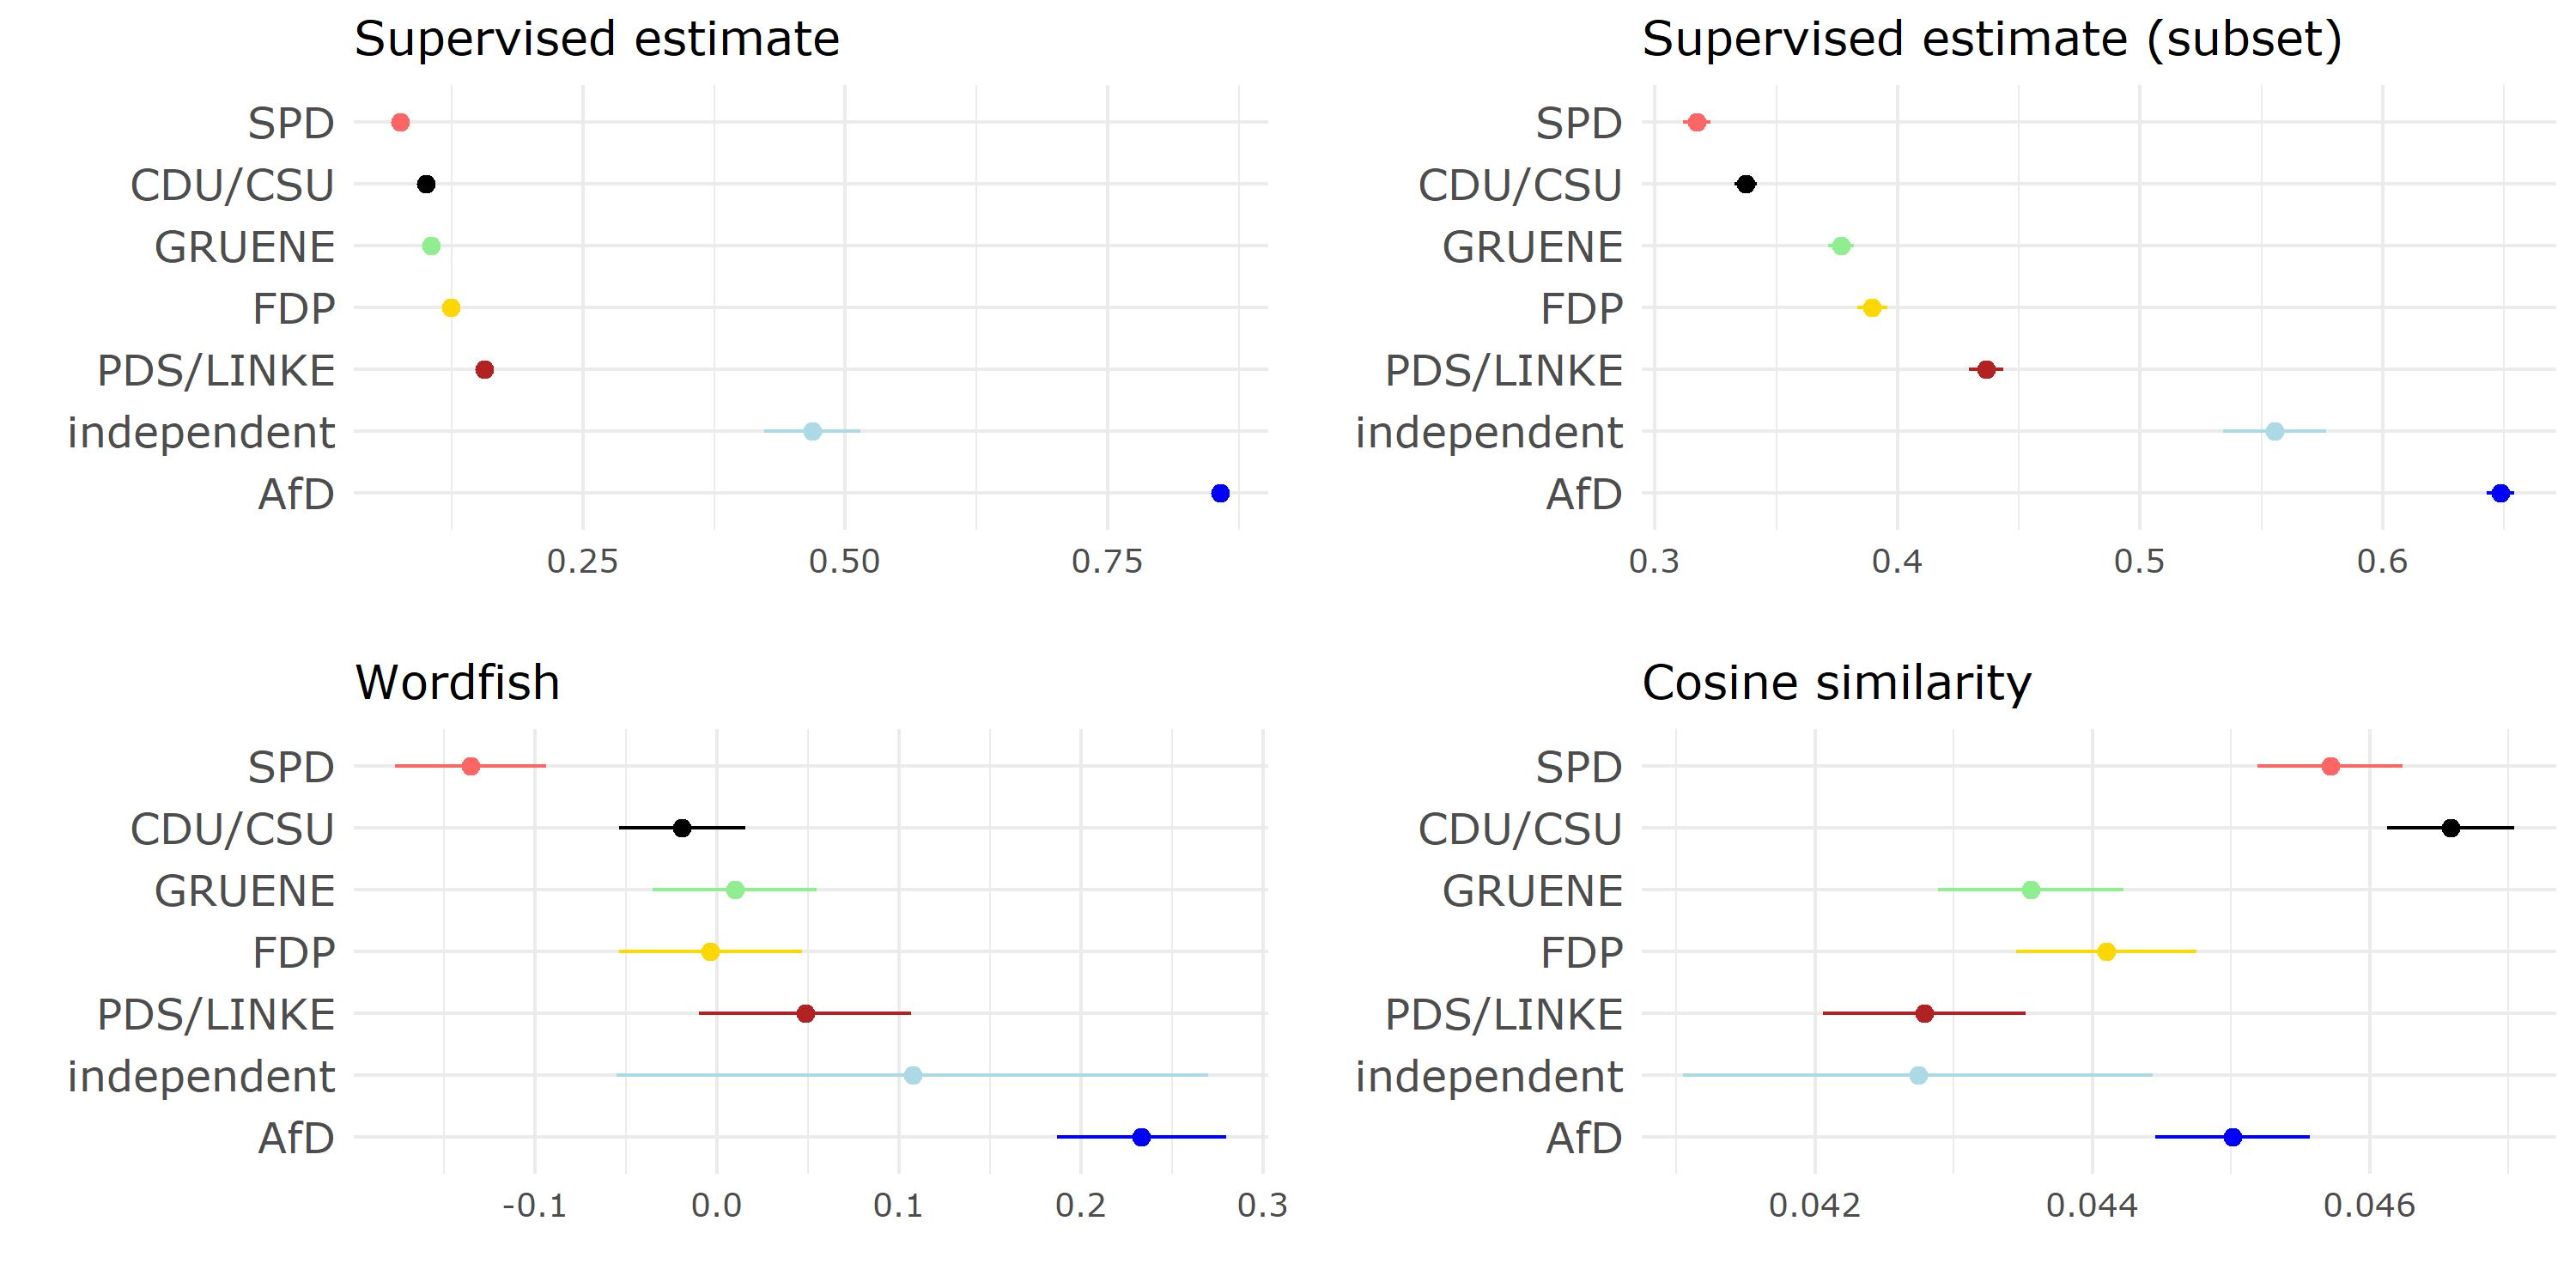
\includegraphics[width = \textwidth]{DE/vis/similarity_pts.jpg}
    \caption{Mean supervised estimates, cosine similarity, and wordfish estimates per party with 95\% confidence intervals. Both wordfish and the restricted supervised estimates (upper right) were trained on a subset of 1000 speeches, which then estimated the positions of all speeches.}
    \label{fig:comp}
\end{figure}

\subsection{Wordfish}

To assess how parties and speakers differ in word use and whether they are more or less similar, a researcher could also use scaling methods. As wordscore (\cite{Laver2003}) requires the selection and labelling of anchor documents, I compare the estimates from the supervised algorithm to wordfish-scores. Wordfish extracts a major underlying dimension which explains differences in word use (\cite{Slapin2008}). The supervised estimates are conceptually different from wordfish estimates. Instead of estimating an underlying dimension explaining differences in word use, the supervised measure estimates a statistical model where word use explains an outcome variable and then employs this model to assess the similarity of documents to the group of interest. Note that using radical-right similarity as the measure of interest likely downplays the conceptual difference of wordfish and supervised estimates, as the AfD is an extreme case, where similarity seems rather correlated with the main underlying factor. This should be different if similarity towards a centrist party were investigated.\par

The last row in figure \ref{fig:comp} shows the wordfish estimates for each party. As the process was too computationally intense to be run with the full set of 11,419 German speeches\footnote{On a machine with 16GB working memory.}, I ran the scaling estimates on a sample of 1,000 speeches with at least 50 words. To make a fair comparison, the upper right graph in \ref{fig:comp} shows the supervised estimates for such a subsample. A first observation is that the wordfish distributions show far more overlap than the supervised estimates\footnote{Note that the sign of the wordfish estimates has been inverted to simplify comparison.}. Other than cosine similarity measures, wordfish places the AfD very distinctly. It also correctly places the independent speakers in proximity to the AfD. Similar to the supervised measures, the distribution does not follow a left-right pattern, but places the governing parties and especially the SPD as most distinct, the opposition parties in between and the independent speakers in proximity to the AfD. However, these estimates also show large confidence intervals and most parties' mean estimates cannot be distinguished. It is only somewhat correlated with the supervised measure (0.17, logged 0.22), although the order of the parties' mean estimates is similar - with the exception of the FDP. \par


Note that this example over-emphasises the conceptual similarity of wordscores and supervised estimates, as I chose the radical-right AfD as an example here. The Wordfish estimates remain identical, whether assessing similarity towards e.g. the Greens or the AfD. The supervised method gives substantial flexibility to the researcher to compare similarities towards different corpora (see case study Austria). Furthermore, the interpretation of the Wordfish scores is harder, as they do not correspond to similarity towards a group (or distinctiveness of that group). Instead, the estimates provide the placement of groups on the best fitting underlying dimension to explain the differences in word use. The interpretation of this dimension is left to the researcher. In this example, there seems to be a mixture of left-right and government-opposition dynamics.\par

Lastly, the runtime of the estimations is also relevant, as researchers want fast analyses that save them time. I compare the runtime of wordfish estimates to that of the oversampling and model fitting for supervised estimates, both for the subsample of 1,000 speeches from the most recent parliamentary session in Germany. Wordfish is estimated using Will Lowe's \texttt{austin}-package for R\footnote{\url{https://conjugateprior.github.io/austin/articles/austin.html}} on Windows; supervised estimates using \texttt{Scikit-Learn} for Python on Linux\footnote{Although wordfish scores could well be estimated with Python and supervised similarity in R (and speed differences partly be caused by these different applications), these platforms reflect the most likely use case for both applications.}. Model fit and prediction for each speech with wordfish took 44 minutes for a sample of 1000 cases (35 minutes for model fit alone). The runtime for oversampling, model fit and generation of supervised estimates was around half a \textit{second} when fitting 1000 speeches, and 3.9 seconds on the full set of 11,419 speeches. Apart from taking far less memory and enabling the estimation of far larger datasets, supervised estimation is about 5,000 times faster than the standard implementation of wordfish.


\section{Conclusion}

The precise measurement of rhetorical similarities is at the heart of many political science questions. This paper presented a novel approach making use of machine learning for the precise and efficient estimation of the similarity of documents to corpora. It allows researchers to estimate how well a given document fits a category of their choosing, compared to a number of other texts. The showcased data demonstrate that supervised estimates provide a valid measure of rhetorical similarity even for longitudinal data with fewer observations. It has also been shown that the estimates produced outperform applications using scaling methods or measures of lexical similarity. \par

The approach is particularly well-suited to study the quality as well as drivers and effects of party accommodation and it was developed with this application in mind. Given that researchers can use virtually any classification of their texts to estimate similarity scores, a plethora of other applications is conceivable. Building on the preliminary findings presented here, a more systematic inquiry might try to predict coalition formations or breakdowns based on the 'signalling' in parties' rhetoric. Vice versa, researchers could assess coalition inclusion probabilities (\cite{Kayser2019Coalition}) and their conditioning effect on accommodation in party rhetoric. The approach could also be exploited to explore the validity of party family classifications by assessing the best predictor words and their underlying dimensions (e.g. through coupling it with factor analysis). That way, it could be established whether members of the same party family in different countries are distinguished by similar language (and thus if parties' classification into the same family is warranted). Scholars of representation might use supervised estimates to assess whether and how certain groups of MPs differ in their political rhetoric, and whether they adapt to their peers across time in office. Given the validity of the estimates even on the speaker-level across time, researchers might apply this to predict party movements in response to leadership changes by assessing a new leaders' position compared to the party preceding the change. \par

Further avenues might also include historical analyses assessing whether certain parties or movements managed to shift public discourse or whether parties have filled opportunity spaces abandoned by other parties. This is particularly of interest given the rise of the radical-right and whether these parties have permanently shifted the political discourse in respective countries (\cite{Wagner2017}). But applications are not restricted to party competition. Peace and conflict scholars might be concerned with insurgent's communication to assess willingness for peace agreements. Communication scholars could explore the similarity of newspapers or corporate leaders to each other.\par

Lastly, two notes of caution. I have shown that supervised estimates excel in comparison to other methods when assessing similarities of documents to corpora. In my application, evidence of the in- and decreasing similarity of established and radical-right parties has been shown. This might nevertheless 'mask' changes in the overall discourse, which might be more or less similar to a certain party. If, for example, a radical-right party's rhetoric has become common among all parties, but the radical-right party has further radicalised to a similar extent, the measure would only capture this within legislative sessions, not for more long-term developments\footnote{I thank Pieter Moens for raising this point.}. If a researcher is interested in how parties affected long-term changes in the political discourse, a similar method might be used, but without training different models for each time-unit.\par

Furthermore, my claim is not that this method is \textit{per se} superior. Instead, practitioners need to select a tool suited to their research interest. The necessity to self-define the outcome of interest gives the researcher considerable flexibility in the application of supervised methods, but also puts the responsibility to properly define the concept of interest in their hands alone. Additionally, established measures might be more advantageous with different research questions. If similarities to single documents are of interest, cosine similarities should be more useful. When instead of similarity, the researcher is concerned with the placement of labels on underlying dimensions explaining differences in word use (e.g. ideology), scaling methods are the way to go. If the researcher's curiosity however revolves around group similarities, supervised estimates should indeed be used. In this way, the paper has contributed to extend the toolbox of empirical social scientists. \par



\section*{Acknowledgements}
This paper was enriched by helpful comments and suggestions by João Areal Neto, Eelco Harteveld, Hauke Licht, Philipp Mendoza, Thomas Meyer, and Gijs Schumacher, as well as the participants of the EPSIP-Colloquium at Humboldt University Berlin and the 2019 ECPR Summer School on Political Parties.


\printbibliography

\newpage

\end{document}